\documentclass[conference]{IEEEtran}
\IEEEoverridecommandlockouts
% The preceding line is only needed to identify funding in the first footnote. If that is unneeded, please comment it out.
\usepackage{cite}
\usepackage{amsmath,amssymb,amsfonts}
\usepackage{algorithmic}
\usepackage{graphicx}
\usepackage{textcomp}
\usepackage{xcolor}
\usepackage{booktabs}
\def\BibTeX{{\rm B\kern-.05em{\sc i\kern-.025em b}\kern-.08em
    T\kern-.1667em\lower.7ex\hbox{E}\kern-.125emX}}
\begin{document}

\title{The Influence of AI Chatbot Interaction Styles on User Acceptance}

\author{\IEEEauthorblockN{Aryan Parajuli}
	\IEEEauthorblockA{\textit{FB5: Department of Electrical Engineering and Computer Science} \\
		\textit{Master of Science - Information Technology}\\
		Lemgo, Germany \\
		aryan.parajuli@stud.th-owl.de}}

\maketitle

\begin{abstract}
	This study provides a comprehensive overview of different interaction styles of an AI chatbot and how it impacts the overall acceptance of AI by its users. It explores features like anthropomorphism and how it influences the user experience towards AI chatbots. The research explores the hypothesis that the AI chatbots having human-like or anthropomorphic responses are likely to be accepted. [Placeholder.....]
\end{abstract}

\begin{IEEEkeywords}
	AI, Chatbots, Human-like, Anthropomorphism, Human-AI Interaction (HAII), User Acceptance
\end{IEEEkeywords}

\section{Introduction}
AI chatbots are used in a large scale recently, due to developments in AI and machine learning. They represent interactive systems in which Human-Computer-Interaction (HCI) takes place and can communicate using natural languages. They are used in diverse sectors like health, education, entertainment, marketing etc. and can imitate human behavior and conversational conditions\cite{b1}. \textit{Anthropomorphism is defined as the assignment of human-like traits, behaviours, or mental states to non-human entities like objects, brands, animals, and, recently, technological devices.} The psychological anthropomorphic characteristics of an AI chatbot along with its empathetic and interactive capabilities makes it more likely to be accepted by a user\cite{b2}. This study analyses the impact of different interaction styles of AI chatbots, focusing mainly on anthropomorphic interaction style and how it influences user acceptance. Based on survey data to investigate user preferences towards this interaction style, contribution of factors like trust, engagement and satisfaction for the overall acceptance is examined. To guide this investigation, the research question is: What is the influence of different interaction styles of AI chatbots on User Acceptance? The hypothesis theorized is: Users tend to show higher acceptance towards AI chatbots with anthropomorphic interaction styles.

\section{Literature Review}

\subsection{Human-AI Interaction (HAII).}
The rise in AI-driven technologies has transitioned typical HCI to a newer field called Human-AI Interaction (HAII) which focuses on the study of interaction between AI computing systems and humans. HAII is dependent on two key factors: Human-AI fit which means how well an AI meets physical, cognitive and emotional needs, and Task-AI fit which means an AI’s capability to perform certain tasks. Depending on a user’s needs and tasks, HAII ranges from full human control to full AI control\cite{b3}. The previous works related to HAII focused primarily on intermittent interaction style which is a turn-taking process where the interaction occurs between the AI system and the user in turns. It is a process where the user constantly provides input and evaluates the feedback from the system until the final goal is achieved. However, new studies highlight continuous interaction style, which is a process where the AI system handles user input in real time and provides ongoing feedback throughout the task. This allows the user to stay focused while the AI assists without interrupting the workflow. Similarly, proactive interaction style is presented where the AI system autonomously initiates and completes actions based on contextual data. This shifts the user's role from actively performing tasks to reacting to or adjusting the system's automated decisions. The HCI community has not broadly engaged with the ideas of continuous and proactive HAII whereas intermittent HAII is already a widely established concept\cite{b4}.

\subsection{Human-Likeliness or Anthropomorphism in an AI-Chatbot.}
An AI-Chatbot or Conversational Agent (CA) can be perceived as human-like if it can conversate using natural language. A study shows that when participants were presented with simulated conversations between an AI and a user across different contexts, they were more likely to judge the AI as a human-like teammate under the conditions that they saw more conversations with it, they were less afraid of robots, and they trusted others more in general. Human-like characteristics of the AI deemed it to be more trustworthy, helpful and acceptable\cite{b5}.The chatbots that mimic certain human traits like showing emotions or empathy, are likely to influence satisfaction, engagement and trust in different ways. Studies show that, an anthropomorphic chatbot can adjust its responses to better align with user expectations which creates a sense of understanding the user. Features such as emojis, active listening, or conversational tone make interactions feel more natural and relatable which increases the user’s willingness to engage. Traits like assertiveness or social-oriented communication, can appear more trustworthy because they seem more capable of building relationships\cite{b6}\cite{b7}\cite{b8}. Similarly, research by Euodia Louis\cite{b9}, mentions about source interactivity which is the ability of users to customize and have control over a platform via interactive features. It highlights studies about how interactivity and customization of AI Chatbots increases user engagement and satisfaction. AI Chatbots like Bing Copilot and ChatGPT allow users to adjust their conversational style to be more context-oriented and human-like and also adjust their responses according to user input. The one-way passive chat room scenario where the user starts a conversation is changed by this engagement between humans and AI chatbots. This makes interactions feel more authentic because AI Chatbots imitate human-conversational flexibility which is an anthropomorphic behavior.

\subsection{Cultural Differences in User Acceptance of AI Chatbots.}
Cultural differences play a crucial role in technology acceptance, impacting key factors like perceived usefulness and ease of use, as outlined by the Technology Acceptance Model (TAM) and the Unified Theory of Acceptance and Use of Technology (UTAUT). Studies by Zakour\cite{b10}, and Srite and Karhanna\cite{b11}, show that cultural dimensions such as individualism, collectivism, power distance, and uncertainty avoidance influence technology acceptance. In terms of chatbots, these cultural factors affect how users perceive interaction styles. Research by Van der Goot and Pilgrim\cite{b12}, found that while both younger and older users are motivated by convenience, their needs for human contact and perceptions of security differ. These findings suggest that chatbot designs should account for cultural differences to enhance user acceptance\cite{b13}. Similarly, studies by Liu and Sundar\cite{b14}, show that empathy and humour enhance user satisfaction and support user interaction. Fahdil and Schiavo\cite{b15}, point out that a medical assistant that uses humorous or satirical approach was able to get a higher patient engagement. Although, humour is a universal approach, it is bound along with culture and language. It differs from culture to culture. A study conducted on empathy, humour and culture in conversational AI chatbots for second language acquisition shows that cultural dimensions improve communication, and culturally aware humour and empathetic responses resulted in positive experiences. Adding cultural nuances to AI chatbots helps for a wider socio-economic and cultural context which broadens user acceptance\cite{b16}.

\section{Methodology}
The study used a wide range of survey data from 415 participants coming from diverse backgrounds. To establish a relation between the interaction style of the AI chatbot and user acceptance, we used relevant questions measured using the Likert scale which provided results in the form of interval data. We also provided an example of two different AI Chatbot responses, one anthropomorphic and the other non-anthropomorphic to evaluate the preference of the participants. We filtered the data because the response from 115 participants was invalid, and the final sample size was reduced to 300 participants.   
\begin{table}[ht]
    \centering
    \caption{Gender Frequency Table}
    \label{tab:genderTest}
    \begin{tabular}{lrr}
        \toprule
        \textbf{Gender} & \textbf{Participants} & \textbf{Total} \\
        \midrule
        Female & 118 & 300 \\
        Male & 180 & 300 \\
        Diverse & 2 & 300 \\
        \bottomrule
    \end{tabular}
\end{table}
\\

Based on table 1, there were 180 male participants, 118 female participants and 2 diverse participants. Besides the gender difference, the major responses came from the people below the age of 30, with significantly fewer responses from those above the age of 30. The highest number of participants, 172 were from the IT or Technological sectors whereas the remaining were from other professional sectors.

\begin{table}[ht]
    \centering
    \caption{Educational Attainment Frequency Table}
    \label{tab:educationalTest}
    \begin{tabular}{lrr}
        \toprule
        \textbf{Education} & \textbf{Participants} & \textbf{Total} \\
        \midrule
        Secondary Education/ High School & 35 & 300 \\
		Vocational Training & 8 & 300 \\
        Bachelor's or equivalent & 191 & 300 \\
        Master's or equivalent & 62 & 300 \\
		Doctorate or equivalent & 1 & 300 \\
		Missing & 3 & 300 \\
        \bottomrule
    \end{tabular}
\end{table}


Table 2 shows the distribution of participants based on their educational attainment, with the highest number of participants, 191 with a bachelor’s degree followed by 62 participants with a master’s degree. The lowest involvement was shown by PHD holders with a single participant. Apart from the difference in educational level, participants were from various religious backgrounds, with Hinduism on the top of the list with 103 participants, followed by Christianity with 77 participants whereas 32 participants did not follow any religion. This range of participants enables us to obtain a broad spectrum of user experiences which offers valuable insights into how AI chatbot interaction styles are perceived across different sociocultural backgrounds.

\begin{table}[ht]
    \centering
    \caption{AI Chatbot Response Preference Frequency Table}
    \label{tab:anthropomorphicTest}
    \begin{tabular}{lrr}
        \toprule
        \textbf{Response} & \textbf{Participants} & \textbf{Total} \\
        \midrule
        Anthropomorphic style response & 197 & 300 \\
		Non-anthropomorphic style response & 103 & 300 \\
        \bottomrule
    \end{tabular}
\end{table}

We provided the participants with examples of anthropomorphic and non-anthropomorphic responses. As shown in table 3, 197 participants preferred the anthropomorphic response whereas 103 preferred the non-anthropomorphic response. Besides this, we also provided 6 quantitative questions to evaluate the likeliness of participants to prefer a specific type of response. 2 questions were inclined towards non-anthropomorphic AI chatbots whereas 4 towards anthropomorphic AI chatbots. We then calculated the mean of the 6 questions as the anthropomorphic preference score. Reverse encoding for the non-anthropomorphic response questions was carried out to ensure that we received accurate average score. \par
The study examined the responses using statistical analysis with JASP (Jeffreys's Amazing Statistics Program). We used analytical methods like the independent samples t-test, emphasizing on the preference of anthropomorphism. We used this particular method because the study aims to compare the anthropomorphic preference score which is the mean value of two independent sample groups where the first group prefers the anthropomorphic response while the second group prefers the non-anthropomorphic response. The data used as the measure for the independent variable is categorical or non-numeric with two levels; anthropomorphic and non-anthropomorphic, whereas the data used as the measure for the dependent variable is the anthropomorphic preference score which is continuous or numerical; derived as the average from the interval scale responses. \\

\section{Results}
\begin{table}[h]
	\centering
	\caption{Independent Samples T-Test}
	\label{tab:independentSamplesT-Test}
	{
		\begin{tabular}{lrrr}
			\toprule
			$ $ & t & df & p  \\
			\cmidrule[0.4pt]{1-4}
			anthropomorphic\_preference\_score & $6.887$ & $141.685$ & $<$ .001  \\
			\bottomrule
			\addlinespace[1ex]
			\multicolumn{4}{p{0.5\linewidth}}{\textit{Note.} Welch's t-test.} \\
		\end{tabular}
	}
\end{table}

Table 4 shows the results of the independent samples t-test. We used Welch’s t-test because there are unequal variances between groups as indicated by the p-value \textless 0.05 from the Brown-Forsythe test for equality of variances. The t-value is 6.887 which indicates that there is a statistically significant difference between the two independent groups where the anthropomorphic group has a higher mean score. The degrees of freedom (df) is 141.685 which is fractional and indicates that Welch’s t-test was used to adjust the unequal variances. A larger df value indicates a reliable test and a good sample size. The p-value is extremely small (p\textless0.001) which shows a high statistical significance and a strong support towards our hypothesis. The probability that this result is obtained by chance is less likely (\textless 0.1\%).                 


\begin{table}[h]
    \centering
    \caption{Independent Samples T-Test with Effect Size}
    \label{tab:independentSamplesT-TestCohensD}
    \resizebox{\linewidth}{!}{ % Adjust table width
        \begin{tabular}{lrrrrr}
            \toprule
            $ $ & t & df & p & Cohen's d & SE Cohen's d \\
            \cmidrule[0.2pt]{1-6}
            anthropomorphic\_preference\_score & $6.887$ & $141.685$ & $<$ .001 & $0.899$ & $0.130$  \\
            \bottomrule
        \end{tabular}
    }
\end{table}

In addition to the independent samples t-test, we calculated the effect size through Cohen’s d which quantifies the effect size and provides insights into the practical significance of the results by determining the magnitude of the difference between the two groups. Table 5 shows that the Cohen’s d value for the anthropomorphic preference score was 0.899 which indicates a large effect size because an effect size of 0.8 or greater is considered to be large. This shows that the difference in mean preference score between anthropomorphic and non-anthropomorphic interaction style groups is noteworthy. The standard error of Cohen’s d was 0.130 which represents the precision of the estimated effect size. The combination of a significant t-test and a large Cohen's d value supports our hypothesis.

\begin{table}[h]
    \centering
    \caption{Regression Coefficients Table}
    \label{tab:regressionCoefficientsTable}
    \resizebox{\linewidth}{!}{ % Adjust table width
        \begin{tabular}{lrrrrr}
            \toprule
            Predictor & Unstandardized Coefficient & Standard Error & Standardized Coefficient & p-value \\
            \cmidrule[0.2pt]{1-5}
            Interaction Style & -0.436 & 0.063 & -0.374 & $<$ .001 \\
            Age  & -0.135 & 0.056 & -0.135 & 0.015 \\
            Education & 0.076  & 0.034 & 0.122  & 0.027 \\
            \bottomrule
        \end{tabular}
    }
\end{table}

\begin{table}[h]
    \centering
    \caption{Regression Model Summary Table}
    \label{tab:regressionModelSummaryTable}
        \begin{tabular}{lrrrrr}
            \toprule
            Metric & Value  \\
            \cmidrule[0.4pt]{1-2}
            $R^2$ & 0.209 \\
            Adjusted $R^2$  & 0.192 \\
            F-Statistic & 12.239\\
            p-value & $<$ .001 \\
            \bottomrule
        \end{tabular}
\end{table}

\begin{figure}[h]
    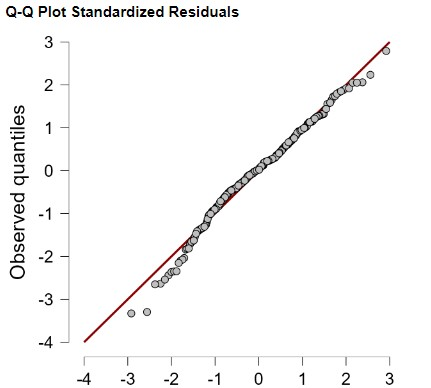
\includegraphics[width=\linewidth]{images/Q-Q Plots for residuals.jpg}
    \caption{Q-Q Plots standardized residuals}
    \label{q_qplots}    
  \end{figure}

  We performed a multiple regression analysis to investigate the influence of interaction styles and certain demographic variables on user acceptance. The adjusted \( R^2 \) value was 0.192 which indicates that the model significantly explained 19.2\% of the variance in user acceptance (\( F\text{-statistic} = 12.239, p < .001 \)) as shown in Table 7. Table 6 shows that the interaction style was highly significant with a \( p\text{-value} < 0.001 \) associating anthropomorphic interaction style with high user acceptance scores. Age and Education were significant predictors among the demographic variables where age negatively associated with user acceptance (\( p = 0.015 \)) which indicates that older participants showed slightly lower preference and education positively associated with user acceptance (\( p = 0.027 \)) which indicates that highly educated participants showed higher acceptance. Gender, Religion and Profession did not significantly impact user acceptance (\( p > 0.05 \)). The Figure 1 shows a Q-Q plot which confirmed that residuals followed a normal distribution which validated the assumptions of the regression model.
  \section{Discussion}
 [Some placeholder text]

\section{Conclusion}
 [Some placeholder text]


\begin{thebibliography}{00}
	\bibitem{b1} L. Nicolescu and M. T. Tudorache, ``Human-Computer Interaction in Customer Service: The Experience with AI Chatbots—A Systematic Literature Review,'' Electronics, vol. 11, no. 10, Article 1579, 2022. [Online]. Available: https://www.mdpi.com/2079-9292/11/10/1579
	\bibitem{b2} C. Pelau, D.-C. Dabija, and I. Ene, ``What makes an AI device human-like? The role of interaction quality, empathy and perceived psychological anthropomorphic characteristics in the acceptance of artificial intelligence in the service industry,'' Computers in Human Behavior, vol. 122, p. 106855, 2021. [Online]. Available: https://www.sciencedirect.com/science/article/pii/S0747563221001783
	\bibitem{b3} Y. Sun, X.-L. Shen, and K. Z. K. Zhang, ``Human-AI interaction,'' Data and Information Management, vol. 7, no. 3, p. 100048, 2023, Special Issue on Human-AI Interaction. [Online]. Available: https://www.sciencedirect.com/science/article/pii/S2543925123000220
	\bibitem{b4} N. van Berkel, M. B. Skov, and J. Kjeldskov, ``Human-AI interaction: intermittent, continuous, and proactive,'' Interactions, vol. 28, no. 6, pp. 67–71, Nov.–Dec. 2021. [Online]. Available: https://doi.org/10.1145/3486941
	\bibitem{b5} J. W. Bonny and K. T. Wynne, ``Increasing Human-Likeness and Acceptance of Conversational Autonomy through Experience,'' in *Proc. 2024 IEEE 4th Int. Conf. Human-Machine Systems (ICHMS)*, 2024, pp. 1–6. [Online]. Available: https://doi.org/10.1109/ICHMS59971.2024.10555683
	\bibitem{b6} A. Rapp, L. Curti, and A. Boldi, ``The human side of human-chatbot interaction: A systematic literature review of ten years of research on text-based chatbots,'' International Journal of Human-Computer Studies, vol. 151, p. 102630, 2021. [Online]. Available: https://www.sciencedirect.com/science/article/pii/S1071581921000483
    \bibitem{b7} A. Fadhil, G. Schiavo, Y. Wang, and B. A. Yilma, ``The effect of emojis when interacting with conversational interface assisted health coaching system,'' in *Proceedings of the 12th EAI International Conference on Pervasive Computing Technologies for Healthcare*, 2018, pp. 378--383.
    \bibitem{b8} Z. Xiao, M. X. Zhou, W. Chen, H. Yang, and C. Chi, ``If I hear you correctly: Building and evaluating interview chatbots with active listening skills,'' in *Proceedings of the 2020 CHI Conference on Human Factors in Computing Systems*, 2020, pp. 1--14.
	\bibitem{b9} E. Louis, ``Exploring User-Desired Interaction in Conversational Generative AI Chatbots,'' Dissertation, Uppsala University, 2024. [Online]. Available: https://urn.kb.se/resolve?urn=urn:nbn:se:uu:diva-531834.
    \bibitem{b10} A. B. Zakour, ``Cultural differences and information technology acceptance,'' in *Proceedings of the 7th Annual Conference of the Southern Association for Information Systems*, Feb. 2004, pp. 156–161.
    \bibitem{b11} M. Srite, ``Culture as an explanation of technology acceptance differences: An empirical investigation of Chinese and US users,'' *Australasian Journal of Information Systems*, vol. 14, 2006. [Online]. Available: https://doi.org/10.3127/ajis.v14i1.4
	\bibitem{b12} M. J. van der Goot and T. Pilgrim, ``Exploring age differences in motivations for and acceptance of chatbot communication in a customer service context,'' in *Chatbot Research and Design*, A. Følstad, T. Araujo, S. Papadopoulos, E. L.-C. Law, O.-C. Granmo, E. Luger, and P. B. Brandtzaeg, Eds. Springer International Publishing, 2020, pp. 173–186.
	\bibitem{b13} D. Dobrowsky, L. Aunimo, G. Thirsty, I. Pezenka, and T. Weber, ``The influence of interactional style on affective acceptance in human-chatbot interaction – A literature review,'' in *HHBIC 2021*, Esignals Research, Haaga-Helia Univ. Appl. Sci., 2021. [Online]. Available: http://www.theseus.fi/handle/10024/793466
	\bibitem{b14} B. Liu and S. S. Sundar, ``Should machines express sympathy and empathy? Experiments with a health advice chatbot,'' *Cyberpsychology, Behavior, and Social Networking*, vol. 21, no. 10, pp. 625–636, 2018, doi: 10.1089/cyber.2018.0110. [Online]. Available: https://doi.org/10.1089/cyber.2018.0110.
	\bibitem{b15} A. Fadhil and G. Schiavo, ``Designing for health chatbots,'' *arXiv preprint arXiv:1902.09022*, 2019.
	\bibitem{b16} C. Zhai and S. Wibowo, ``A systematic review on cross-culture, humor and empathy dimensions in conversational chatbots: The case of second language acquisition,'' *Heliyon*, vol. 8, no. 12, 2022. [Online]. Available: https://doi.org/10.1016/j.heliyon.2022.e12056. doi: 10.1016/j.heliyon.2022.e12056.
\end{thebibliography}

\end{document}
